\chapter{PROJETO DE TESTES REALIZADO}
\label{chp:capitulo5}

\section{Métodos}
O propósito inicial dos testes realizados é compreender amplamente o impacto das adições ao programa. Para tal, uma série de métricas foram empregadas para avaliação na execução do programa, de uma maneira exaustiva, para todos os modelos relevantes (excluindo-se apenas o SQLiGOT, por motivos já mencionados). Através dela foi possível obter uma ideia do impacto que os novos modelos têm, e como o wafamole++ se adapta com \textit{wrappers} novos.

O parâmetro principal para tal avaliação foram \textbf{500} execuções por modelo no wafamole++. Tanto os modelos antigos como os modelos novos foram examinados. As medidas bases extraídas foram:
\begin{alineas}
\item \textbf{Número de rodadas restantes} - A partir dessas obtém-se o número de rodadas ou iterações consumidas;
\item \textbf{Menor probabilidade de payload encontrada} - É possível medir com essas a precisão de um determinado modelo;
\item \textbf{Tempo de execução em segundos} - Tanto para o tempo médio de execução como para diagnosticar a robustez. Um tempo maior indica uma maior eficiência em virtude da reforço do dataset;
\item \textbf{Execuções com iterações máximas alcançadas} - Quanto mais ocorrências dessa medida, mais robusto é o modelo uma vez que não é gerado um exemplo adversarial na execução.
\end{alineas}

\bigskip 

\section{Resultados e discussão}

Abaixo segue uma tabela com uma série de informações geradas de relevância, construídas a partir das métricas listadas acima: 

\begin{table}[H]
\centering
\caption{Visão Global de Execuções Realizadas}
\begin{supertabular}{m{4.0cm}m{3.7cm}m{3.6cm}m{3.0cm}}
\hline
\multicolumn{1}{m{4.0cm}|}{\centering{Modelo}} &
\multicolumn{1}{m{3.741cm}|}{\centering{Runtime médio}} &
\multicolumn{1}{m{3.635cm}|}{\centering{Qtd. de Rounds restantes média (arredondado)}} &
\centering\arraybslash{Execuções sem êxito}\\\hline
\centering{\verb+test_ada+} &
\centering{181.5269} &
\centering{334} &
\centering\arraybslash{198}\\
\centering{\verb+test_svc_extra_moled+} &
\centering{8.6750} &
\centering{715} &
\centering\arraybslash{26}\\
\centering{\verb+test_svc_moled+} &
\centering{7.6486} &
\centering{993} &
\centering\arraybslash{16}\\
\centering{\verb+test_svc_no_mole+} &
\centering{2.4484} &
\centering{752} &
\centering\arraybslash{0}\\
\centering{\verb+sgd_trained+} &
\centering{2.3822} &
\centering{988} &
\centering\arraybslash{0}\\
\centering{\verb+test_sgd_wafamole+} &
\centering{2.1332} &
\centering{996} &
\centering\arraybslash{0}\\
\centering{\verb+token_random_forest+} &
\centering{3.0299} &
\centering{986} &
\centering\arraybslash{1}\\
\centering{\verb+token_naive_bayes+} &
\centering{2.7982} &
\centering{969} &
\centering\arraybslash{1}\\
\centering{\verb+token_linear_svm+} &
\centering{2.3284} &
\centering{997} &
\centering\arraybslash{0}\\
\centering{\verb+token_gauss_svm+} &
\centering{2.2002} &
\centering{999} &
\centering\arraybslash{0}\\
\centering{\verb+waf_brain+} &
\centering{3.6010} &
\centering{1000} &
\centering\arraybslash{0}\\
\hline
\end{supertabular}
    \legend{Fonte: Elaboração Própria }
    \label{tab:tests}
\end{table}
\bigskip

Os fatores que indicam uma performance melhor são relativamente contraintuitivos - um \textit{runtime} médio grande indica dificuldade em gerar um exemplo adversarial, que na verdade é um bom indicador para o Web Application Firewall sendo avaliado. Similarmente, poucos rounds restantes ao final da execução apontam para muitas iterações sendo consumidas e um WAF robusto, e um alto número de execuções sem êxito sugere casos em que o Web Application Firewall não se mostra suscetível a um ataque naquela execução. 

Curiosamente, o modelo \verb+test_sgd+ gerado a partir do dataset original do WAF-A-MoLE não apresentou grandes melhorias em comparação com o modelo do dataset \verb+SQLiV3.json+, \verb+sgd_trained+. Acredita-se que seja uma questão de adequação do classificador utilizado, uma vez que com a respectiva substuição do \textit{Stochastic Gradient Descent} pelo \textit{Ada Boost} e virtualmente a mesma implementação o mesmo se torna o WAF mais robusto do wafamole++.

Dado isso, os modelos de maior interesse com base nos dados obtidos certamente são os entitulados de \verb+test_ada+, \verb+svc_extra_moled+, \verb+svc_moled+, \verb+svc_no_mole+. Neles, é possível ver uma melhora nítida em robustez quando comparado aos demais. O primeiro conjunto de \textit{Distribution Plots} amostrado a seguir detalha a evolução da robustez do Firewall alvo em função dos reforços incrementados ao dataset (indicados por \verb+no_mole+ como sem reforço, \verb+moled+ para um conjunto pequeno de reforço e \verb+extra_moled+ para um conjunto ainda maior de reforço), além de comparar com o modelo \verb+test_ada+ para perspectiva. 

\begin{figure}[ht]
    \centering
    \caption{Distribution plot de tempos de execução (em segundos)}
    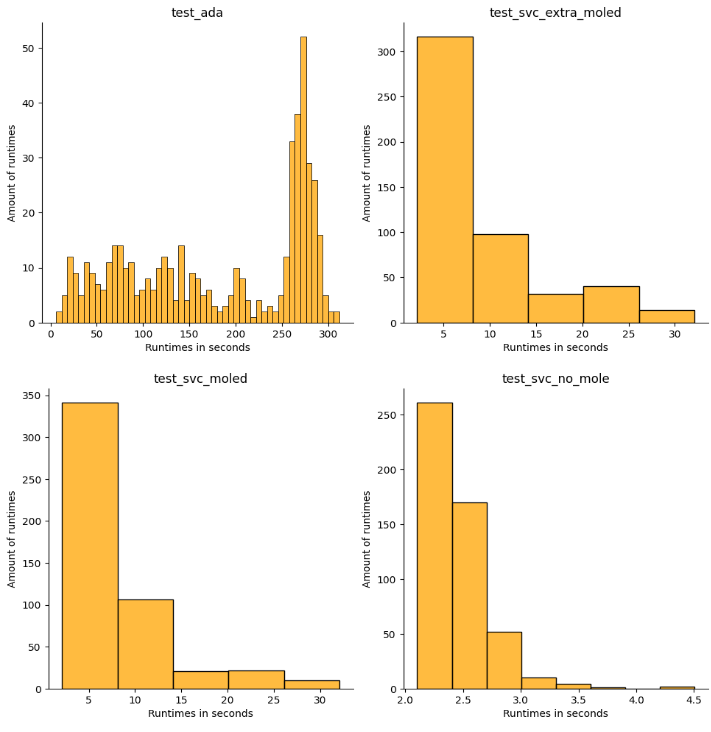
\includegraphics[width=18cm]{figuras/graficos/runtimes_amount_set1.png} 
    \legend{Fonte: Elaboração Própria}
    \label{fig:mole-evolution} 
\end{figure}

Atentando-se aos valores no eixo das abscissas, é possível identificar que os tempos de execução ficam consideravelmente maiores conforme os reforços são aplicados ao modelo \verb+test_svc+. Somado a isso, uma diferença radical pode ser avaliada no modelo \verb+test_ada+, com a maioria dos tempos de execução levando uma quantia consideravelmente maior do que todos os modelos avaliados. Isso aponta para uma performance próxima do \verb+SQLiGOT+, um modelo virtualmente inacessível por exigir muito do WAF-A-MoLE e de código fechado.

Para melhor ilustrar a amplitude de tempos de execução, a distribuição dos mesmos foi mapeada em um gráfico \textit{Box plot}, agrupada por cada modelo. O único caso não contemplado é um \textit{outlier} no modelo \verb+token_random_forest+, que fora omitido para não comprometer a visualização do gráfico. Foi também feita uma separação entre o \verb+test_ada+ e os demais modelos, uma vez que seu intervalo é distinto o suficiente para distorcer as proporções.

\begin{figure}[ht]
    \centering
    \caption{Box plot de distribuição tempos de execução (em segundos), por modelo}
    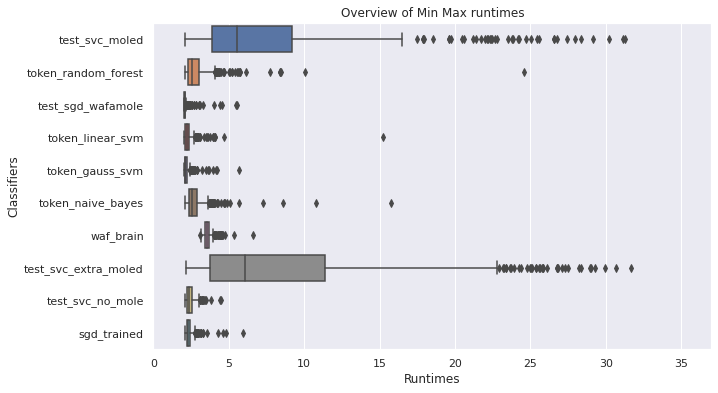
\includegraphics[width=18cm]{figuras/graficos/min_max_all.png} 
    \legend{Fonte: Elaboração Própria}
    \label{fig:min-max-all} 
\end{figure}

\begin{figure}[ht]
    \centering
    \caption{Box plot de distribuição tempos de execução (em segundos), para modelo Ada Boost}
    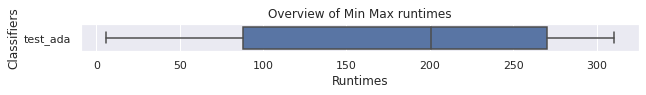
\includegraphics[width=18cm]{figuras/graficos/min_max_ada.png} 
    \legend{Fonte: Elaboração Própria}
    \label{fig:min-max-ada} 
\end{figure}

Sumariamente, esses resultados permitem compreender que o classificador \textit{Stochastic Gradient Descent} possivelmente não é o mais indicado para esse tipo de modelagem, com um desempenho semelhante independente do banco usado para treiná-lo. Não obstante, fica estabelecida a capacidade de aprimoramento que os modelos gerados pelo wafamole++ e WAF-A-MoLE oferecem a determinados dataset de treinamento. Espera-se que a abordagem deste trabalho sendo transparente permita resultados ainda mais enriquecedores de modelos novos em um breve futuro.

% reminder {figure}[H] forces positioning!
